\chapter{Bedrijfsachtergrond}
\section{De onderneming}
Opgericht in 1995, door huidig CEO J. (Jan) Kaptijn en wijlen C. (Chris) Goos met het innovatieve idee om een geselecteerd assortiment visproducten aan te bieden over de hele wereld zonder zelf ook maar een enkele visverwerkingsband te moeten aanschaffen. Seafood Connection werkt nauw samen met landen over de hele wereld om lokaal visproducten aan te kunnen bieden met een hoge kwaliteitsstandaard. Deze standaard wordt gegarandeerd door contacten van het bedrijf zelf, grondige controles uit te laten voeren bij de leveranciers op locatie en het productie- en verwerkingsproces te houden aan hoge Europese standaarden als IFS, BRC, MSC en HACCP. \citep{sfcreglement}

In 2013 werd de meerderheid van Seafood Connection Holding gekocht door het Japanse Maruha Nichiro. Dit miljardenbedrijf, opgericht in 1880, is evenals SFC in alle uithoeken van de wereld te vinden. SFC hoopt met deze samenwerking te kunnen profiteren van de kennis en middelen van Maruha Nichiro, die naast de verkoop van visproducten het doel hebben om de hele waardeketen van de visindustrie te domineren. Dit betekent dat Maruha Nichiro een hand heeft in een groot aantal bedrijven dat rijkt van bedrijven in de aquacultuur, distributiecentrums en fabrieksschepen. Het moederbedrijf houdt het Nederlandse Seafood Connection nauwlettend in de gaten, dit doet zij door werknemers van Maruha Nichiro bij Seafood Connection op locatie te laten werken zodat zij periodieke rapportage kunnen versturen naar het hoofdkantoor in Japan. \citep{sfcwebsite,Visserijnieuws}

\begin{figure}[!hb]
    \centering
    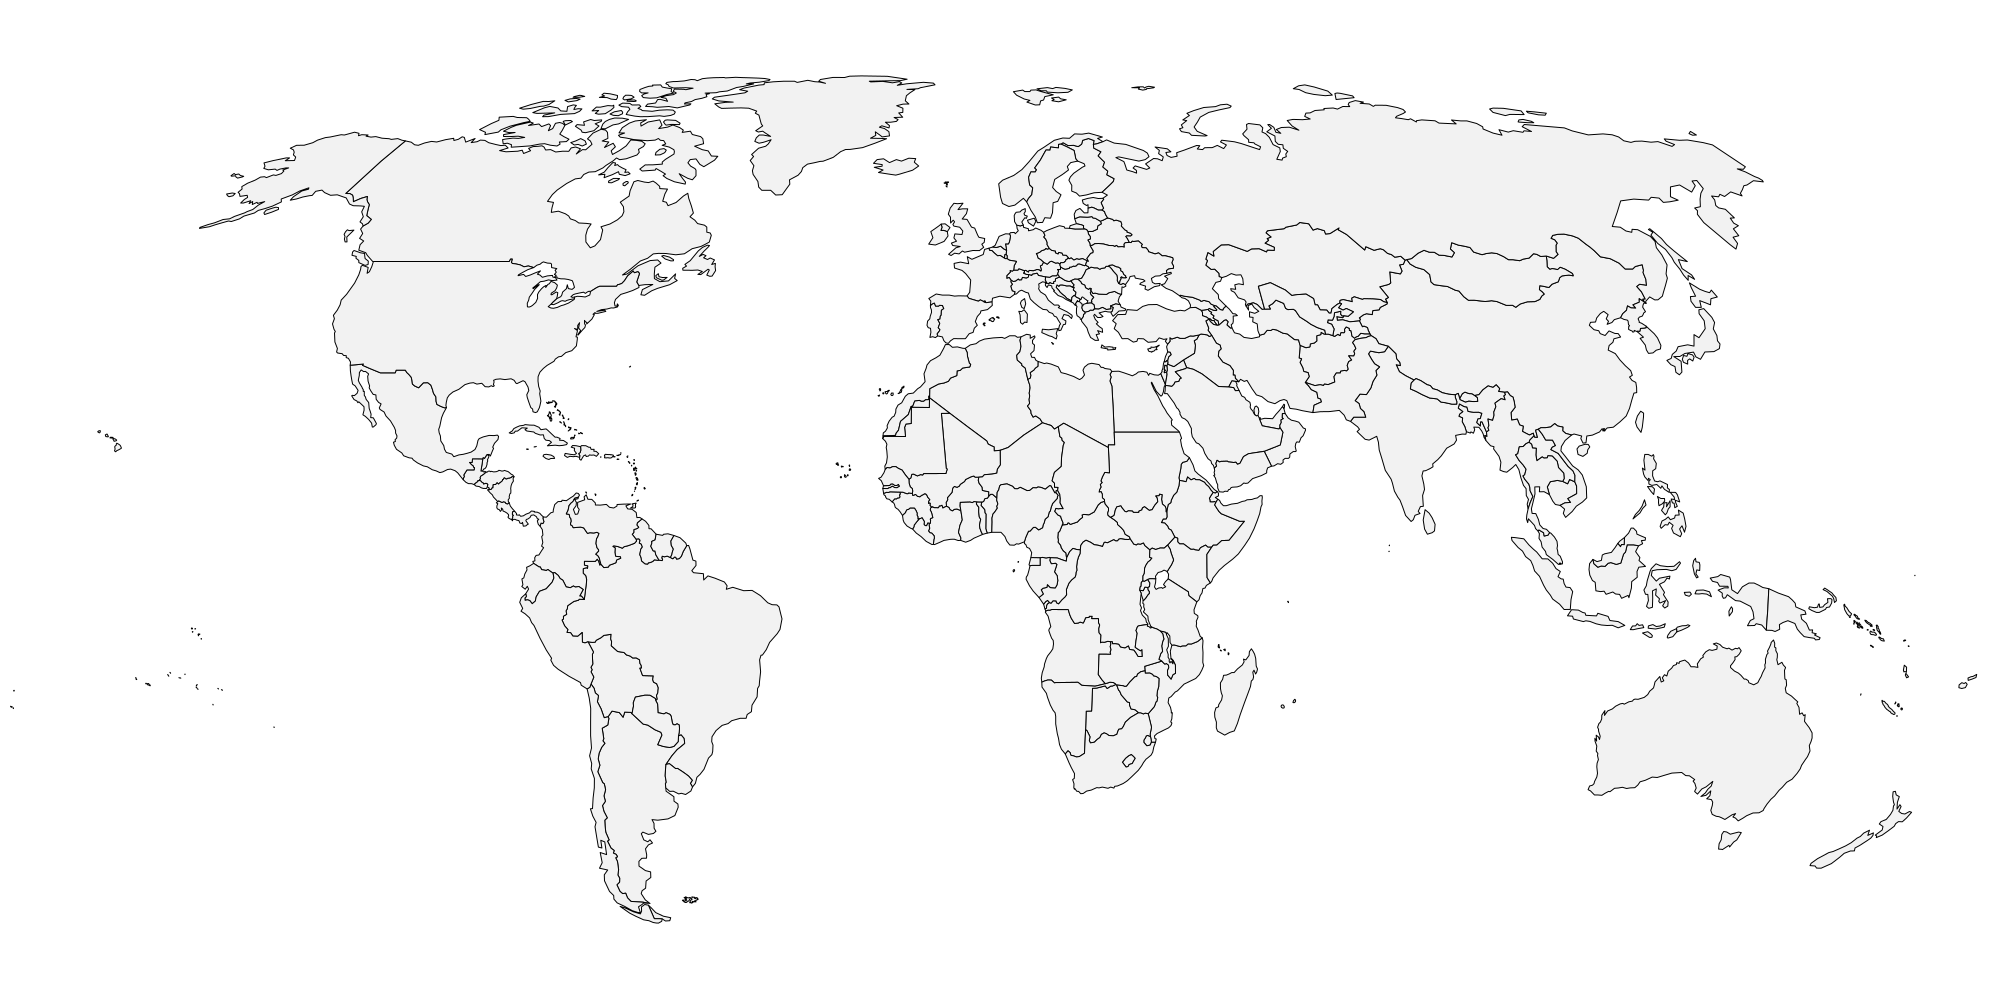
\includegraphics[width=0.5\textwidth]{kaart}
    \caption{Alle kantoren van Seafood Connection en moederbedrijf Maruha Nichiro \citep{sfcwebsite}}
    \label{fig:kantorensfc}
\end{figure}

\label{beschr:activiteiten}
Het is voor een bedrijf als SFC aantrekkelijk om relatief veel schulden op zich te nemen ten opzichte van haar bezittingen. SFC koopt grootschalig in voor verscheidene producten op een groot aantal markten. Dit betekent dat wanneer een grote hoeveelheid visproducten worden gekocht, het gebruikelijk is dat de levering doorgaans pas na één maand plaatsvindt. Na levering blijft de voorraad doorgaans twee maanden op voorraad voor het verkocht wordt, waarbij betaling van deze order één tot twee maanden na de aflevering van deze goederen plaatsvindt. De duur van deze fasen verschilt per markt en product maar de strekking hier van is dat Seafood Connection in feite pas haar geld terug ontvangt tussen vier tot zelfs zes maanden na inkoop van het product. \citep{quickscan}

\begin{figure}[!h]
    \centering
    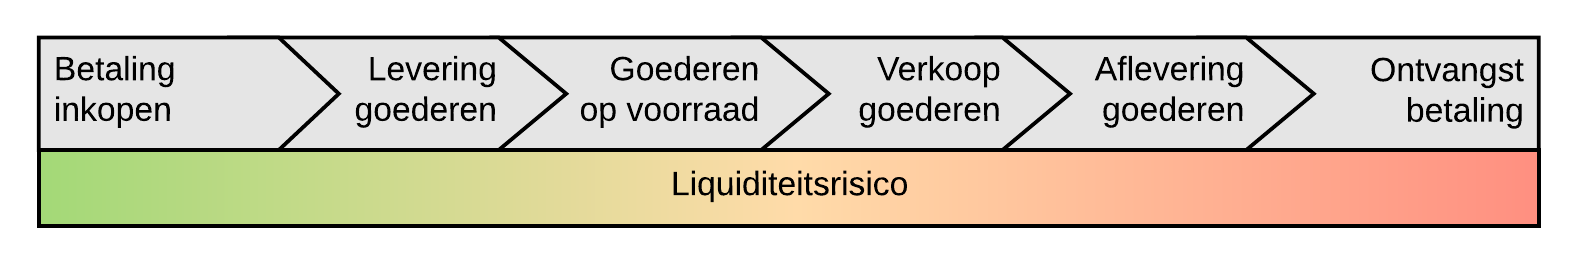
\includegraphics[width=\textwidth]{liquiditeitsrisico}
    \caption{Liquiditeitsrisico en druk op de schulden gedurende het bedrijfsproces}
    \label{fig:liquiditeitsrisico}
\end{figure}


\section{De organisatie}
Seafood Connection is een handelsbedrijf in diverse diepvries visproducten met daarnaast in beperkte mate doorstroom van eigen goederen met een eenvoudig, technisch omzettingsproces \citep{aoibsfc}. Voor de verschillende bedrijfsactiviteiten fungeert Seafood Connection als:

\begin{enumerate}
    \item Handelsbedrijf dat hoofdzakelijk aan andere bedrijven levert
    \item Productiebedrijf met homogene massaproductie
    \item In zeer beperkte mate dienstverlening aan derden (door commissie op verkopen aan derden)
\end{enumerate}

Seafood Connection is vijftig gemotiveerde werknemers sterk. Het kantoor op Urk vervult alle bedrijfsfuncties grotendeels op één locatie; er zijn enkele medewerkers werkzaam bij een klein, lokaal productieproces, namelijk bij de zagerij van Coldstore Urk waar een groot deel van de voorraad van SFC zich bevindt. De organisatie heeft vier niveaus: het managementteam (MT) dat de strategie formuleert, de unitmanagers (UMO) die hun afdelingen aansturen, managers die het aanspreekpunt zijn voor hun deelprocessen in de verschillende afdelingen, én assistants die de afdelingen ondersteunen met verschillende werkzaamheden. SFC is een \gls{lsorganisatie} met een gedeelde P-, G-, en M-indeling opgedeeld in de afdelingen: inkoop, opslag, verkoop, finance, ICT and production, HRM, compliance, en marketing verdeeld over vier segmenten: wholesale, retail, industry, en group companies (geografisch beheer). \citep{quickscan,sfcreglement}

\section{De branche}
Kenmerken voor succes in de branche zijn ogenschijnlijk het hebben van een affiniteit voor duurzaamheid, naleving van kwaliteitsstandaarden en goed toegankelijk zijn zodat visproducten in elk jaargetijde geleverd kunnen worden. In mindere mate is er ook sprake van prijsconcurrentie, omdat alle visverwerkers uit dezelfde vaargebieden de vis vangen. 

Seafood Connection is niet de enige aanbieder van vis. SFC opereert op Urk, één van de grootste centrums voor de visverwerking in Nederland, de CFO van Seafood Connection zegt hier zelf over dat het een gezonde hoeveelheid concurrentie voor de kiezen heeft. Het is dan ook niet verrassend dat de onderneming als grootste succescriteria heeft gekozen om te winnen in de markt, dit plaatst zij boven criteria als het beschikken over een zo uniek en nieuw mogelijk productassortiment of efficiënte bedrijfsvoering. 

De missie van Seafood Connection is om het volgende te anticiperen: klantbelangen, de behoefte aan duurzame visproducten, en nieuwe trends. De onderneming wil dit realiseren door nieuwe partners te verkrijgen in cruciale markten in Europa, Amerika en Azië. Tevens worden nieuwe keteninnovaties verkregen door fusies en overnames in de visindustrie. \citep{sfcwebsite}